\section{Anwedungen des Satzes von Kutta-Joukowski}
\label{joukowski:anwendungen}

\subsection{Magnus Effekt}
\begin{figure}
	\centering
	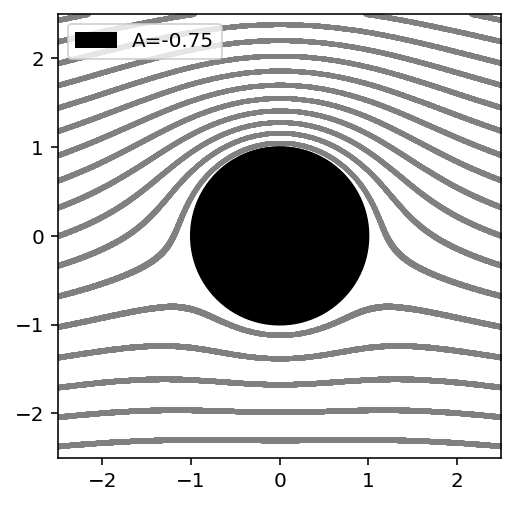
\includegraphics[width=0.45\textwidth]{papers/joukowski/images/05_stroemungslinien/Magnus_Strom_A075_g.png}
	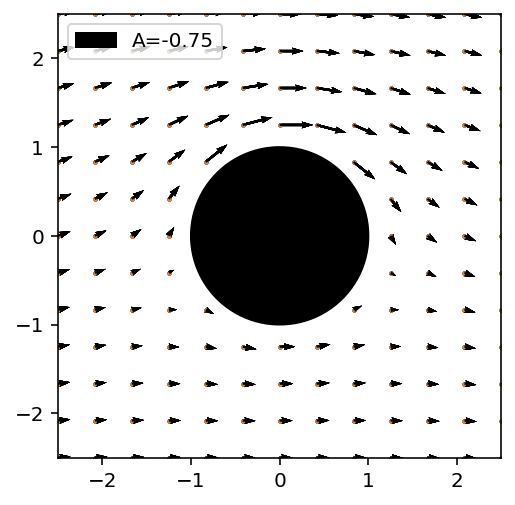
\includegraphics[width=0.45\textwidth]{papers/joukowski/images/05_stroemungslinien/Magnus_Speed_A075.png}
	\caption{
		Durch das Rotieren des Zylinders entsteht eine Asymmetrie in den Strömungslinien.
		Diese Asymmetrie führt dazu,
		dass die Geschwindigkeit ober- und unterhalb des Zylinders nicht mehr gleichmässig zunehmen.
		\label{joukowski:Stroemungslinien:fig_magnus}
	}
\end{figure}

Bei rotierenden Zylindern entsteht eine Kraft, sofern eine Luftströmung existiert. Dieser Effekt kann beispielsweise eingesetzt werden, um den Kraftstoffverbrauch von Schiffen zu senken.

Grafisch lässt sich dieser Effekt aufzeigen, indem die Funktion $f(z)$ aus Beispiel~\ref{joukowski:stroemungslinien:beispiel:joukowski-transformation} 
zum Ausdruck
\begin{equation}
	\label{joukowski:Stroemungslinien:equation_magnus}
	f(z) = v_\infty \cdot \biggl(z+ \frac{1}{z}\biggr) - i\cdot A\cdot \log(z)
\end{equation}
erweitert wird.
Mit dem Parameter $A$ kann der Effekt eines rotierenden Zylinders in einem Strömungsfeld gesteuert werden.
Der rotierende Zylinder führt dazu, dass die Luft ebenfalls zirkuliert.
Mit dem Parameter $A$
kann somit direkt Einfluss auf die Zirkulation genommen werden.
Wird der Parameter $A$ beispielsweise auf $-0.75$ gesetzt, resultiert ein Strömungs- und Geschwindigkeitsfeld wie in Abbildung ~\ref{joukowski:Stroemungslinien:fig_magnus}.
Anhand der Abbildung der Geschwindigkeitsvektoren kann erkannt werden,
dass oberhalb des rotierenden Zylinders die Strömung eine höhere Geschwindigkeit aufweist wie unterhalb.
Höhere Geschwindigkeit bedeutet tieferer Druck und somit eine Auftriebskraft.

Leiten wir die Funktion $f(z)$ nach $z$ ab, erhalten wir
\[
	\overline{v(z)}
	=
	v_{\infty} \cdot \biggl(1 - \frac{1}{z^2}\biggr) 
	- \frac{i \cdot A}{z}.
\]
Sortieren wir die Terme nach ihren Potenzen von $z$ im Nenner erhalten wir
\[
	\overline{v(z)}
	=
	v_{\infty} - \frac{i \cdot A}{z} - \frac{v_{\infty}}{z^2}.
\]
Vergleichen wir dies mit dem Reihenausdruck~\eqref{joukowski:komplexe-analysis:original-laurent-reihe},
sehen wir, dass nur die ersten drei Terme vorkommen.
Aus Satz~\ref{joukowski:komplexe-analysis:satz:zirkulation} ist uns aber bekannt, dass nur der Term
\[
	\frac{a_1}{z}
\]
einen Beitrag leistet.
Daraus folgt aus der Gleichung~\eqref{joukowski:komplexe-analysis:zirkulation-berechnet}
\[
	\Gamma
	=
	2 \pi i \cdot (-i \cdot A)
	=
	2 \pi A
\]
Setzen wir unser Resultat für $\Gamma$ in den Satz von Kutta-Joukowski ein
erhalten wir für die komplex konjugierte Kraft
\[
	\overline{F'}
	=
	i \rho v_{\infty} 2 \pi A.
\]
Es folgt eine reine Auftriebskraft mit dem Ausdruck
\[
	F'_y
	=
	-\rho v_{\infty} 2 \pi A.
\]

\subsection{Tragflügel}
\begin{figure}
	\centering
	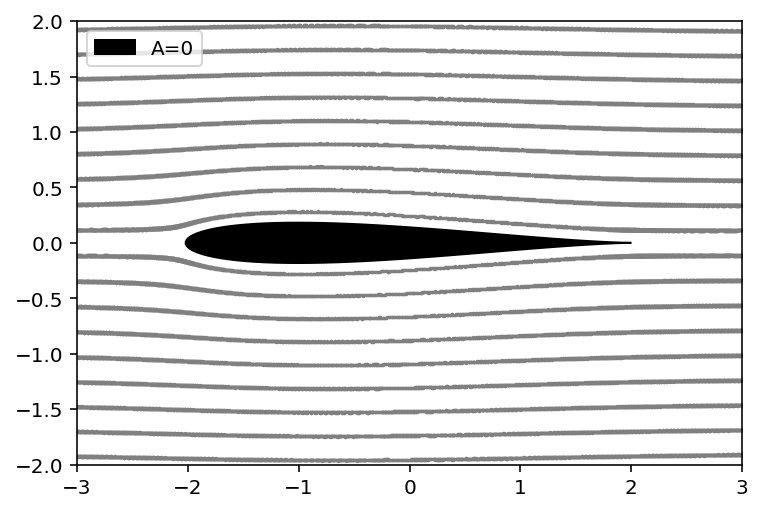
\includegraphics[width=0.6\textwidth]{papers/joukowski/images/05_stroemungslinien/fluegel_strom_A000_V04_g.png}
	\caption{
		Das flügelprofil ist in sich symmetrisch, was dazu führt dass die Strömungslinien auch symmetrisch verlaufen.
		Diese Anordnung produziert so keine Auftriebskraft.
		\label{joukowski:Stroemungslinien:fig_fluegel1}
	}
\end{figure}

\begin{figure}
	\centering
	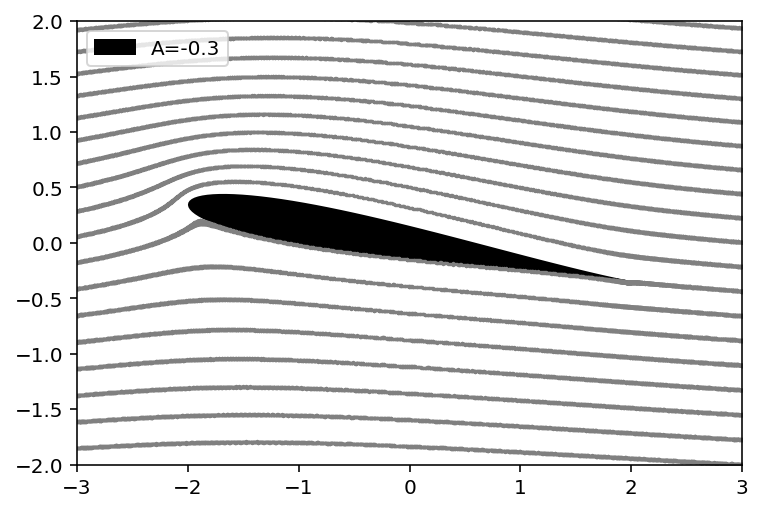
\includegraphics[width=0.6\textwidth]{papers/joukowski/images/05_stroemungslinien/fluegel_strom_A030_Rot_V02_g.png}
	\caption{
		Das Flügelprofil weist einen Anstellwinkel auf. Somit
		verschwindet die Symmetrie in den Strömungslinien und es entsteht eine Auftriebskraft,
		obwohl das Flügelprofil symmetrisch ist.
		\label{joukowski:Stroemungslinien:fig_fluegel2}
	}
\end{figure}

Nun haben wir bereits viel über Geschwindigkeiten und Strömungen gesprochen.
Die interessante Frage ist jedoch, was das alles mit einem Flügelprofil zu tun hat.
Ein Einheitskreis kann relativ einfach so transformiert werden, dass er einem an der reellen Achse symmetrischen Flügelprofil entspricht.
Hierzu braucht es lediglich eine Verschiebung mit kleinem Realanteil und anschlissend erneut die Transformation $z + \frac{1}{z}$. Eben diese Transformation wird die Kutta-Joukowski Transformation genannt.
Da Strömungslinien holomorph sind, können auch diese transformiert werden.

In Abbildung ~\eqref{joukowski:Stroemungslinien:fig_fluegel1} wird ein symmetrisches Flügelprofil gezeigt. Dieses erzeugt zunächst keinen Auftrieb und dient lediglich zu Anschauungszwecken.

Abbildung ~\eqref{joukowski:Stroemungslinien:fig_fluegel2} entspricht einem Flügelprofil mit Anstellwinkel.
Hierzu muss der transformierte Flügel in der komplexen Ebene im Uhrzeigersinn rotiert werden.~
Damit die Strömungslinien der Realität entsprechen, muss der Faktor $A$ in Gleichung ~\eqref{joukowski:Stroemungslinien:equation_magnus} passend gewählt werden. Dies haben wir numerisch mithilfe unserer Visualisierung ermittelt.
Mit diesem Modell können wir die Strömungslinien um ein Flügelprofil ermitteln.
Es wird ausserdem deutlich, dass dieser Flügel Auftrieb generieren muss, da eine Asymmetrie in den Strömungslinien entsteht.
